\section{Introduction}
In this chapter, we discuss the inspection strategy for DFO methods, with an emphasis on filling the gap between global and local optimization strategies.
When the objective function is non-convex and has spurious local minima, it is generally very challenging to find the global minimum.
In such cases, both global and local DFO methods may fail to deliver a satisfactory solution, as global method may be too computationally expensive and local methods may be trapped in a local minima.

We delve into the dichotomy between these two optimization strategies and discuss the $R$-local optimization approach \cite{chen2019run}, designed to bridge this gap. $R$-local optima lie between local and global optima, and often ensures a suitable solution quality by providing an adjustable radius for the solution's local neighborhood.

We also explore how $R$-local optimization interacts with DFO methods. Despite their advantages, the Run-and-Inspect method, the first proposed $R$-local optimization method, can be computationally expensive, especially when the cost of sampling the objective function is not significantly cheaper than the gradient. However, in the context of DFO, the addition of inspections may not substantially impact the overall sample complexity.

Our proposed framework directs local DFO methods towards an $R$-local minimum, by escaping a local minima if possible. This algorithm that doesn't rely on a global surrogate model, which can be computationally demanding in high-dimensional scenarios. Instead, it can be integrated with any local DFO method that generates a sequence of iterates, thereby capitalizing on the strengths of existing local DFO methods to leverage the known structures of the problem.


\subsection{The gap between global optimization and local optimization}
The majority of the optimization methods are either global optimization or local optimization methods. They approach these problems in very different ways, which creates a gap between them. 

\paragraph{Global Optimization} This class of methods aims to find the absolute best solution (up to a small tolerance) in the \emph{entire} solution space for an optimization problem. In other words, it searches for the overall minimum or maximum. The techniques used for global optimization are typically exhaustive, as they have to explore the entire problem space to ensure they have found the best possible solution up to the tolerance. This is because there may be many local optima, but only one (or a few) global optima. As a result, these methods can be computationally expensive, particularly for complex, high-dimensional problems.

\paragraph{Local Optimization} This class of methods, on the other hand, focuses on finding a good solution in a neighborhood, no matter how small it is, of a specific point in the solution space. This does not necessarily mean that the solution will be the best overall; instead, it means that there is no better solution in some vicinity of the found one. Thus, local optimization methods can be faster and less computationally expensive than global ones, but they may miss the global optimum if it lies outside of the selected neighborhood.

\paragraph{Gap between these two types of optimization} The gap can be understood through the following perspectives.

Global optimization guarantees the best solution, while local optimization only guarantees the best solution within a local neighborhood. However, the size of the neighborhood is not known or controllable.
Due to the need to explore the entire solution space, global optimization usually requires much more computational effort, causing much longer running time, than local optimization.

In practice, the choice between local and global optimization often depends on the specific problem, the resources available, and the acceptable trade-offs. For low-dimensional problems where it is crucial to find the absolute best solution, global optimization becomes necessary. However, for many problems, a solution that is ``good enough'' is sufficient. 

Local methods, despite only producing local solutions, may be preferred and sometimes are only the choice due to their efficiency. 
To improve the solution quality of local methods, meta-heuristics were introduced. They include using multiple starting points, simulated annealing, genetic algorithms that allow occasional moves in the worse direction, etc.
However, neither local methods nor their meta-heuristic improvements could quantify how ``good enough'' their solutions are.

\paragraph{Bridging the gap by $R$-local optimization}
According to \cite{chen2019run}, 
an $R$-local minimizer is a type of local minimizer that specifies a radius of the local neighborhood around the minimizer.

More specifically, suppose we would like to minimize a function $f: \mathbb{R}^n \rightarrow \mathbb{R}$. We say that $x^\star\in\mathbb{R}^n$ is an $R$-local minimizer of $f$ if  that $x^\star$ is a  minimizer of $f$ in the closed ball ${x \in \mathbb{R}^n: \|x - x^\star\| \leq R}$.
This means $x^\star$ is a local minimizer in the neighborhood of radius $R$ around it. 

The concept of an $R$-local minimizer is often used when we want to guarantee the solution found to have a sufficient quality in a vicinity of a defined size. This can be helpful when the global minimizer cannot be easily found or when the function is too complex to optimize over its entire domain. The value of $R$ could be chosen based on some prior knowledge or through a process of trial and error.

% include a figure
\begin{figure}[t]
    \centering
    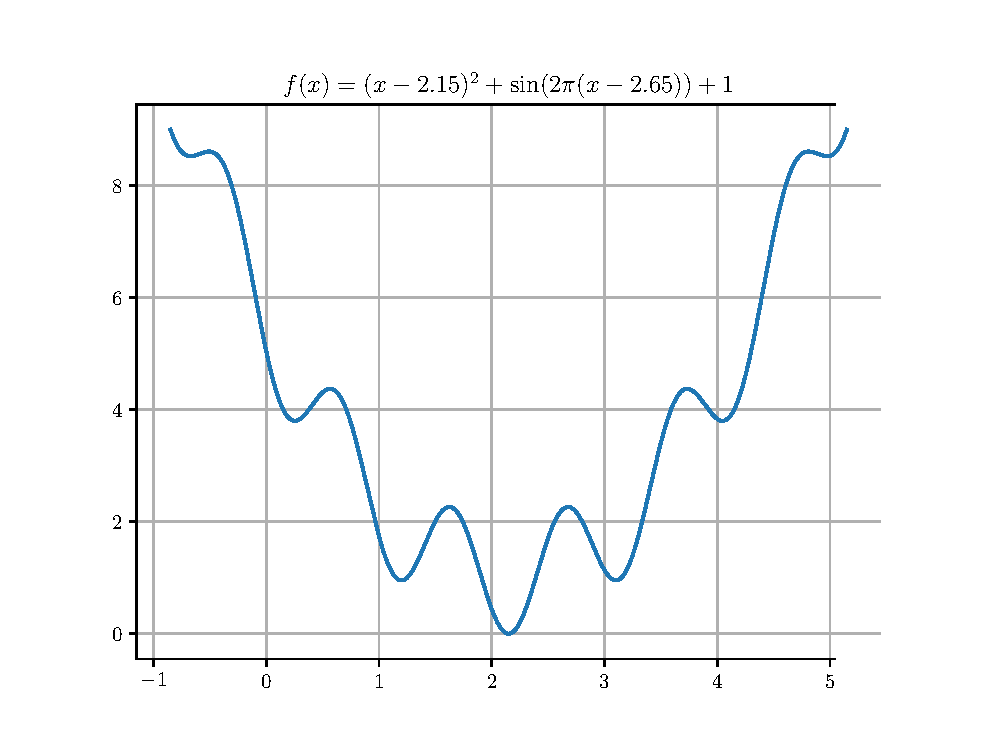
\includegraphics[width=0.6\textwidth]{sin1D.eps}
    \caption{A function with spurious local minima. When $R$ is sufficiently large, an $R$-local minimum is a global minimum.}
    \label{fig: 1D quad + sin}
\end{figure}

\subsection{DFO and $R$-local optimization}
$R$-local optimization offers clear advantages over purely local methods in terms of discovering better solutions. However, it often incurs a higher computational cost to escape from a local minima.
This can become prohibitively expensive in certain scenarios, particularly when the cost of sampling the objective function is not necessarily much lower than its gradient. However, in derivative-free optimization, unless there are special structures (such as sparse gradients described in \cite{cai2020zeroth}), an additional factor of $d$, compared to its gradient-based counterpart, in the sample complexity is unavoidable. Consequently, performing inspections may not significantly impact the overall sample complexity in this case.

\subsection{Assumptions and Notation}
Our proposed method, Inspect-as-you-Run (IR) is a framework that can be applied to any local DFO method that generates a sequence of iterates. 
We assume that the local DFO method $\mathcal{A}$ is given,
and the objective function $f$ satisfies the conditions for $\mathcal{A}$ to converge to a local minimum.
We also assume that $f$ is $\bar{L}$-Lipschitz continuous. Note that, however, if $\nabla f$ is already assumed to be Lipschitz, as in the analyses of many methods, this assumption implies the Lipschitz continuity of $f$.

Also, as in the previous chapter, let $\| \cdot \|$ denote the Euclidean norm, $\unif(S)$ be the uniform distribution over $S$, and the unit sphere be written as $\mathcal{S}^{d-1}$. In addition, the closed ball of radius $R$ centered at $x$ is denoted as $B(x, R) = \{y \in \mathbb{R}^d : \|y - x\| \leq R\}$.

We then introduce a notion of an approximate $R$-local minimizer, which generalizes the $R$-local minimizer:
\begin{definition} \label{def: approximate R-local minimizer}
    Given a descent threshold $\nu$, a point $\bar{x}$ is said to be an \emph{approximate $R$-local minimizer} if $f(\bar{x}) \leq f(x) + \nu$ for all $x \in B(\bar{x}, R)$.    
\end{definition}

Furthermore, defining the following notion of trapping would be useful, because we want to restrict how far the iterates wander around while we inspect nearby points.
\begin{definition}
    Let $\{x_k\}_{k=0}^{K}$ be a sequence in $\mathbb{R}^d$. We say $\{x_k\}$ is trapped in a $D$-ball for $k_0 \leq k \leq k_1$ if $\|x_{k} - x_{k^{\prime}}\| \leq D$ for all $k_0 \leq k, k^{\prime} \leq k_1$.
\end{definition}

